\section{Introdução}
Este documento guia o gerenciamento e o planejamento do desenvolvimento 
do protótipo de software do Projeto Kanban. Ele define a organização do projeto, 
as práticas de gerenciamento adotadas (baseadas no método Kanban), 
o quadro e os cartões utilizados, além dos marcos do projeto.

\section{Organização do Projeto}
A equipe de desenvolvimento é composta pelos seguintes membros, os quais desempenharam, 
na sua grande maioria, os papéis que dizem respeito a elaboração dos documentos:
\begin{itemize}
    \item \textbf{Marcus Vinicius Balbino Cavalcante}
    \item \textbf{Gustavo Macedo}
\end{itemize}

\section{Práticas de Projeto e Gerenciamento (Método Kanban)}
O gerenciamento do projeto adota o \textbf{Método Kanban}. O progresso 
será acompanhado visualmente por meio de um quadro Kanban, permitindo 
o fluxo contínuo de entrega de valor e limitação do trabalho 
em andamento (WIP).

\subsection{Quadro Kanban}
O quadro Kanban criado para o projeto inicialmente era composto pelas colunas:
"A FAZER", "FAZENDO" e "FEITO". No entanto, notou-se a necessidade da adição de 
subdivisões nas colunas para melhor organização das atividades. Foi visto ao 
longo do desenvolvimento que era preciso ter uma coluna do tipo "buffer" entre 
a coluna "FAZENDO" e "FEITO" para armazenar as atividades que foram concluídas, 
mas que ainda não foram validadas, e uma coluna "BACKLOG" para armazenar os
cartões de ideias futuras ao próprio projeto. Assim, criamos as colunas "REVISÃO", 
e a coluna "DO PROJETO", respectivamente. Além disso, usaremos raias para separar 
as atividades para os membros do grupo.


\subsubsection{Colunas do Quadro Kanban}
\begin{itemize}
    \item \textbf{BACKLOG}: Propósito - Fila de opções que contém ideias 
    sobre o projeto.
    \item \textbf{A FAZER}: Propósito - Armazena as atividades (cartões) 
    que foram mapeadas e aguardam disponibilidade da equipe para serem 
    iniciadas.
    \item \textbf{FAZENDO}: Propósito - Contém os cartões em que a equipe 
    está trabalhando ativamente no momento. Esta coluna possui um limite de 
    Work-in-Progress (WIP) para evitar gargalos.
    \item \textbf{REVISÃO}: Propósito - Armazena as atividades (cartões) 
    que foram concluídas, mas que ainda não foram validadas.
    \item \textbf{FEITO}: Propósito - Recebe os cartões cujas atividades foram 
    totalmente concluídas e validadas, prontas para entrega ou já entregues.
\end{itemize}



\subsection{Cartões Kanban (Simulação)}
Os cartões utilizados para gerenciar as tarefas contêm as seguintes 
informações: identificador, nome, responsável, data limite para término, 
prioridade e descrição. Como simulação da construção deste projeto, os 
documentos entregáveis e as funcionalidades do protótipo foram divididos em 
cartões organizados nas tabelas a seguir.

\begin{table}[H]
    \centering
    \caption{Cartões de Documentação (Entregáveis)}
    \vspace{0.3cm}
    \resizebox{\textwidth}{!}{
    \begin{tabular}{|l|l|l|l|l|p{6cm}|}
        \hline
        \textbf{ID} & \textbf{Nome} & \textbf{Responsável} & \textbf{Data} & \textbf{Prio.} & \textbf{Descrição} \\ \hline
        Doc-001 & Processo de gerenciamento & Marcus V. & 12/05/2026 & Alta & Descrição do gerenciamento, quadro e cartões usados. \\ \hline
        Doc-002 & Visão e escopo & Marcus V. & 14/05/2026 & Alta & Elaboração do documento de visão e escopo (vision). \\ \hline
        Doc-003 & Requisitos não funcionais & Marcus V. & 17/05/2026 & Média & Especificação de requisitos não funcionais. \\ \hline
        Doc-004 & Histórias de usuário & Marcus V. & 20/05/2026 & Alta & Especificação de requisitos funcionais (user story). \\ \hline
        Doc-005 & Arquitetura do software & Gustavo M. & 24/05/2026 & Alta & Descrição da arquitetura (architecture notebook). \\ \hline
        Doc-006 & Projeto de interface & Gustavo M. & 28/05/2026 & Alta & Storyboards e wireframes da interface com usuário. \\ \hline
        Doc-007 & Projeto físico de BD & Gustavo M. & 01/06/2026 & Alta & Diagrama e texto do banco de dados físico. \\ \hline
        Doc-008 & Infraestrutura & Gustavo M. & 04/06/2026 & Média & Descrição de implantação, hardware, software e serviços. \\ \hline
    \end{tabular}
    }
\end{table}

\begin{table}[H]
    \centering
    \caption{Cartões de Desenvolvimento (Protótipo)}
    \vspace{0.3cm}
    \resizebox{\textwidth}{!}{
    \begin{tabular}{|l|l|l|l|l|p{6cm}|}
        \hline
        \textbf{ID} & \textbf{Nome} & \textbf{Responsável} & \textbf{Data} & \textbf{Prio.} & \textbf{Descrição} \\ \hline
        Dev-001 & Configuração Inicial & Marcus V. & 06/06/2026 & Alta & Setup do repositório, dependências e infraestrutura base. \\ \hline
        Dev-002 & CRUD Quadros e Raias & Gustavo M. & 10/06/2026 & Alta & Serviços para criar, ler, atualizar e excluir quadros e raias. \\ \hline
        Dev-003 & CRUD Cartões & Marcus V. & 12/06/2026 & Alta & Serviços para gerenciar os cartões de atividades. \\ \hline
        Dev-004 & Movimentação & Gustavo M. & 15/06/2026 & Alta & Mover cartões entre colunas/raias e limite WIP. \\ \hline
        Dev-005 & Métricas Kanban & Marcus V. & 17/06/2026 & Média & Cálculo de cycle time, lead time, throughput e WIP. \\ \hline
        Dev-006 & Teste de Sistema & Gustavo M. & 20/06/2026 & Alta & Gravação de vídeo demonstrando cenário de sucesso. \\ \hline
        Dev-007 & Empacotamento ZIP & Marcus V. & 21/06/2026 & Alta & Fechamento do protótipo e documentos no arquivo final. \\ \hline
    \end{tabular}
    }
\end{table}

\begin{figure}[H]
    \centering
    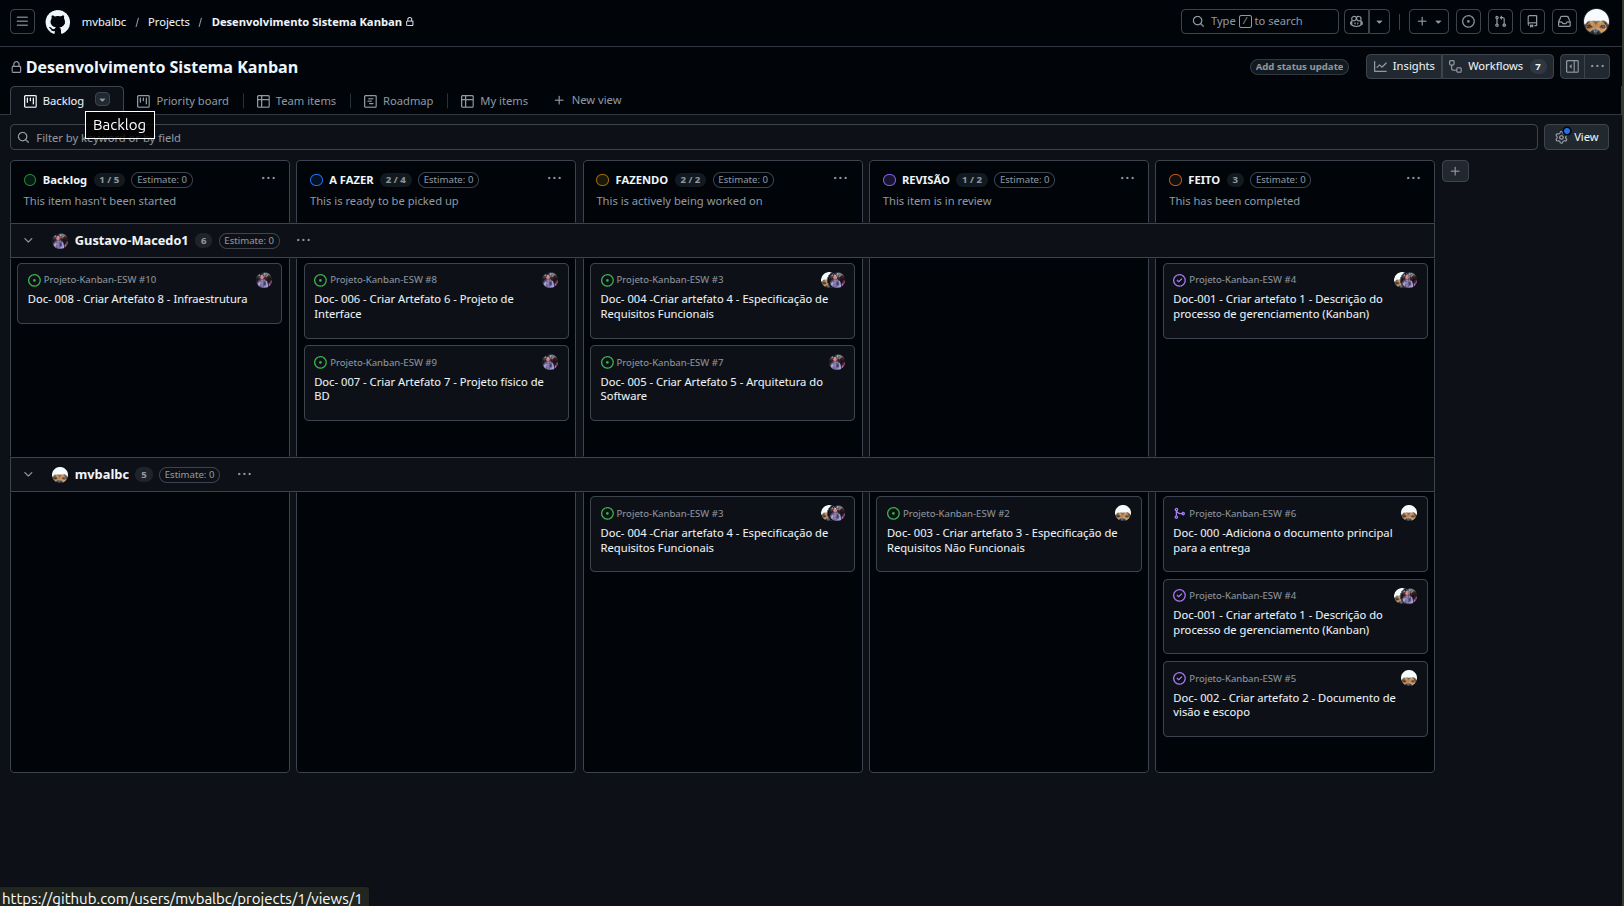
\includegraphics[width=1.0\textwidth]{../DocsLaTeX/images/quadro_kanban.png}
    \caption{Quadro Kanban do Projeto }
\end{figure}

\begin{figure}[H]
    \centering
    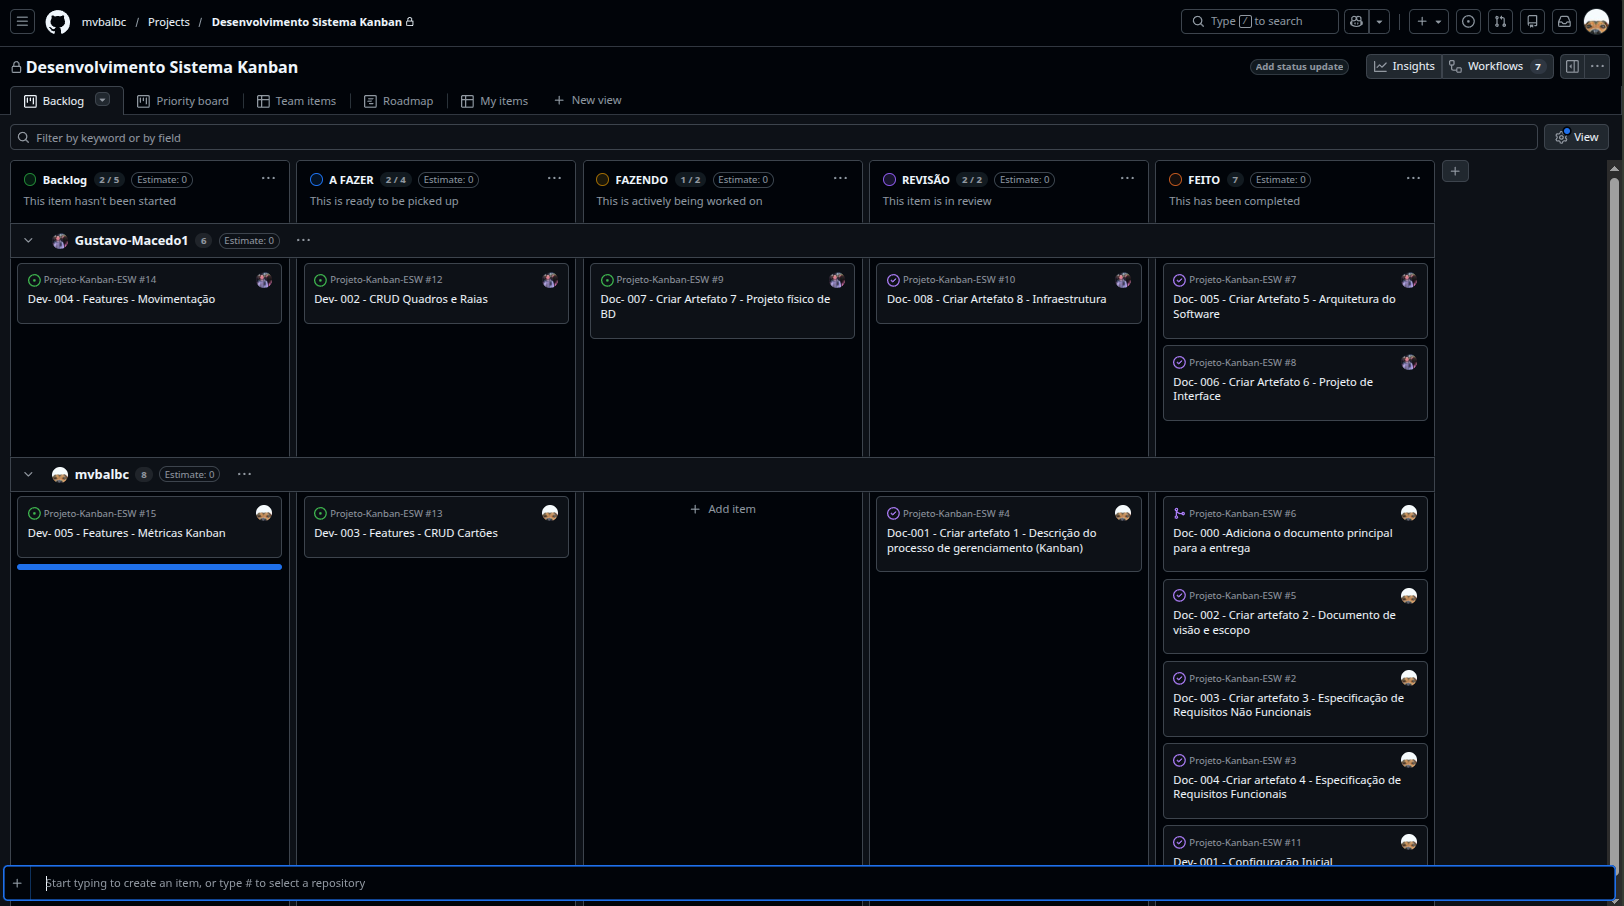
\includegraphics[width=1.0\textwidth]{../DocsLaTeX/images/quadro_kanban2.png}
    \caption{Quadro Kanban do Projeto em fase de desenvolvimento do protótipo.}
\end{figure}

\subsubsection{Políticas de Fluxo e Limites de WIP}
Para garantir a eficiência do método, adotamos um limite de WIP 
(Work-in-Progress) igual a 2 na coluna "FAZENDO". Isso significa 
que os dois membros da equipe não podem puxar novas tarefas se 
já houverem duas atividades em execução simultânea. 
A transição para a coluna "REVISÃO" exige que o código 
sofra um Code Review ou que o documento seja revisado 
pelo membro que não o redigiu, garantindo a validação 
cruzada antes do estado "FEITO".

